\chapter{The Evaluation of Deep Graph Networks} \label{ch:evaluation-dgns}
Over the years, \glspl{dgn} have yielded strong performances on several predictive tasks, becoming the \defacto learning tool for graph-related problems. Given their appeal, several \gls{dgn} architectures have been developed recently. These architectures need to undergo a thorough evaluation to understand which one is better suited for a certain task. The evaluation requires both an extensive model selection phase, to select appropriate hyper-parameters, as well as a model evaluation phase to obtain an estimation of the generalization ability of the network. In the literature, the evaluation of \glspl{dgn} is carried out on a variety of benchmark datasets, generally from the chemistry and social sciences domains, where graphs are used to represent molecules and social networks, respectively. However, as pointed out by researchers \citep{shchur2018pitfalls}, the papers that introduce novel architectures often adopt not reproducible or unfair experimental setups, which make the comparisons among models unreliable. Moreover, there is a tendency of attributing improved performances to subtle architectural changes, when in reality the improvement is a consequence of a more extensive model selection \cite{lipton2018troubling}. In this section, we present three contributions related to address these important issues in the context of \glspl{dgn}. Specifically, we:
\begin{itemize}
    \item provide a rigorous evaluation of existing \glspl{dgn} models in the context of graph classification, using a standardized and reproducible experimental environment. Specifically, we perform a large number of experiments within a rigorous model selection and assessment framework, in which all models are compared using the same node features and data splits;
    \item investigate if and to what extent current \gls{dgn} models can effectively exploit graph structure on the evaluation benchmarks. To this end, we also evaluate two domain-specific structure-agnostic baselines, whose purpose is to disentangle the contribution of structural information from node features;
    \item study the effect of node degrees as features in social datasets. We show that adding node degrees to the node features can be beneficial, and it has implications as to how many convolutional layers are needed to obtain good performances.
\end{itemize}

\section{Datasets}
All the chosen graph  datasets are  publicly  available \citep{kersting2016benchmark}  and  represent  a  relevant subset of those most frequently used benchmarks in the literature to compare \glspl{dgn}. Some collect molecular graphs, while others contain social graphs. Specifically, we use the following chemical datasets:
\begin{itemize}
    \item D\&D \citep{dobson2003dd} is a graph dataset in which nodes are amino acids, and there is an edge between two nodes if they are they are neighbors in the amino-acid sequence or in 3D space. The task is a binary classification one, where the objective is to determine whether a graph represents an enzyme or non-enzyme;
    \item PROTEINS \citep{borgwardt2005proteins} is a subset of D\&D where the largest graphs have been removed;
    \item NCI1 \citep{wale2008nci1} is a dataset made of chemical compounds screened for ability to suppress or inhibit the growth of a panel of human tumor cell lines. The task is a binary classification one, where the objective is to determine if a chemical compound acts as suppressor or inhibitor;
    \item ENZYMES is a dataset of enzymes taken from the BRENDA enzyme database \citep{schomburg2004enzymes}. In this case, the task is to correctly assign each enzyme to one out of 6 Enzyme Commission (EC) numbers.
\end{itemize}
As regards datasets containing social graphs, we use the following:
\begin{itemize}
    \item IMDB-BINARY and IMDB-MULTI \citep{yanardag2015imdbredditcollab} are movie collaboration datasets. Each graph is an ego-network where nodes are actors or actresses, and edges connect two actors/actresses which star in the same movie. Each graph has been extracted from a pre-specified genre of movies, and the task is to classify the genre graph the ego-network is derived from.
    \item REDDIT-5K \citep{yanardag2015imdbredditcollab} is a dataset where each graph represents an online thread on the Reddit platform, and nodes correspond to users. Two nodes are connected by an edge if at least one of the two users commented each other on the thread. The task is to classify each graph to a corresponding community (a sub-reddit);
    \item COLLAB \citep{yanardag2015imdbredditcollab} is a dataset where each graph is an ego-network of different researchers from some research field. There is an edge between two authors if they coauthored a scientific article. The task is to classify each ego-network to the corresponding field of research.
\end{itemize}
All node features are discrete (we shall refer to them as node labels equivalently). The only exception is the ENZYMES dataset, which also has an additional 18 continuous features. The social datasets do not have node features. In this case, we use either an uninformative label for all nodes, or the node degree. Specifically, social datasets are used to understand whether the models are able to learn structural features on their own or not. The statistics of the datasets, which include number of graphs, number of target classes, average number of nodes per graph, average number of nodes per graph, and number of node labels (if any) are reported in Table \ref{tab:comparison-datasets}.
\begin{table}[h!]
    \footnotesize
    \renewcommand\arraystretch{1.1}
    \caption{Dataset Statistics. Note that, when node labels are not present, we either assign the same feature or the degree to all the nodes in the dataset.} \label{tab:comparison-datasets}
    \begin{center}
    \begin{tabular}{c l c c c c c}
    \toprule
    &  & \Thead{Graphs} & \Thead{Classes} & \Thead{Avg. Nodes} & \Thead{Avg. Edges} & \Thead{Labels}\\
    \toprule
    \multirow{4}{*}{\rotatebox[origin=c]{90}{\Thead{\textsc{Chem.}}}}
    &D\&D            & 1178 & 2 & 284.32 & 715.66 & 89 \\
    &ENZYMES       &  600 & 6 &  32.63 &  64.14 &  3 \\
    &NCI1          & 4110 & 2 &  29.87 &  32.30 & 37 \\
    &PROTEINS      & 1113 & 2 &  39.06 &  72.82 &  3 \\
    \midrule
    \multirow{5}{*}{\rotatebox[origin=c]{90}{\Thead{\textsc{Social}}}}
    &COLLAB     & 5000 & 3 & 74.49 & 2457.78 &  - \\
    &IMDB-BINARY   & 1000 & 2 &  19.77 &  96.53 &  - \\
    &IMDB-MULTI    & 1500 & 3 &  13.00 &  65.94 &  - \\
    &REDDIT-BINARY & 2000 & 2 & 429.63 & 497.75 &  - \\
    &REDDIT-5K     & 4999 & 5 & 508.82 & 594.87 &  - \\
    \bottomrule
    \end{tabular}
    \end{center}
\end{table}

\section{Architectures}\label{sec:comparison-architectures}
In total, we choose five different \gls{dgn} architectures. The high-level structure of the \gls{dgn} comprises an input layer, a stack of one or more \glspl{gcl}, a graph readout layer and a final MLP classifier, which maps the graph representation to the dataset-dependent output. Following, we describe in detail the kinds of \gls{gcl} used by the \glspl{dgn}.

\paragraph{Graph Isomorphism Network} The \gls{gin} convolutional layer by \citet{xu2019gin} is implemented as follows:
$$\StateVector{v}{\ell} = \Fun{MLP} \Par{(1 + \epsilon^{(\ell)})\,\Elem{h}{v}^{(\ell-1)} + \sum_{u \in \Neigh(v)} \StateVector{u}{\ell-1}},$$
where $\epsilon \in \Real$ is a trainable parameter, and MLP is a neural network with 2 hidden layers, each one consisting of a linear transformation, followed by a BatchNorm layer and a \gls{relu} non-linearity. The first layer of the \gls{dgn} is not a \gls{gcl}, but a graph readout that sums the node features, and passes them through an MLP identical to the one just described. The graph embedding obtained by this layer is then summed to the graph embeddings computed by the \glspl{gcl}.

\paragraph{GraphSAGE}
The Graph SAmple and aggreGatE (GraphSAGE) layer by \cite{hamilton2017graphsage} is implemented as follows:
$$\StateVector{v}{\ell} = \sigma\Par{\LayerMatrix{w}{\ell}\StateVector{u}{\ell-1} + \frac{1}{|\Neigh(v)|} \LayerMatrix{U}{\ell} \sum_{u \in \Neigh(v)} \StateVector{u}{\ell-1}}.$$
Notice that the original formulation also implements a form of node sampling, since it is applied to large graphs. Here, since the size of the graph we deal with is manageable, we do not implement node sampling.

\paragraph{GraphSAGE + DiffPool}
In order to have a representative \gls{dgn} with pooling, we tested a variant of GraphSAGE, where a DiffPool layer is added to the network after every GraphSAGE convolution. Internally, the DiffPool layer is implemented as in Section \ref{sec:pooling}, where $\Fun{S}_e$ and $\Fun{S}_p$ are a stack of 3 GraphSAGE layers respectively. Thus, one DiffPool layer requires to compute 6 graph convolutions. The number of clusters $k$ is deterministic, and is obtained as $\alpha M$, where $M$ is the maximum number of nodes among the graphs in the dataset, and $\alpha$ is a coarsening factor which is 0.1 if only one DiffPool layer is applied, and 0.25 otherwise.

\paragraph{ECC}
The Edge-Conditioned Convolutional layer by \cite{simonovsky2017ecc} is implemented as follows:
$$\StateVector{v}{\ell} = \sigma\Par{ \frac{1}{|\Neigh(v)|}\sum_{u \in \Neigh(v)} \Fun{MLP}(\Elem{e}{u,v})^{\Transpose} \StateVector{u}{\ell-1}},$$
where MLP is a neural network that computes a weight between the hidden state of the current node $\Elem{h}{v}^{(\ell-1)}$ and its generic neighbor $\StateVector{u}{\ell-1}$, using the edge feature vector as input, composed of one hidden layer with ReLU non-linearities and a subsequent linear output layer. Each convolutional layer of the corresponding \gls{dgn} comprises of a stack of 3 ECC layers.

\paragraph{DGCNN}
The graph convolutional layer of the Deep Graph Convolutional Neural Network (DGCNN) \citep{zhang2018dgcnn}, is the following:
$$\StateVector{v}{\ell} = \Fun{tanh} \Par{\LayerMatrix{w}{\ell} \sum_{u \in \Neigh(v)} \Matrix{D}^{-1}_{vu}\StateVector{u}{\ell-1}},$$
where $\Matrix{D}^{-1}$ is the inverse degree matrix. After all the convolutional layers are applied, the computation is followed by SortPool layer, which performs graph pooling, and a final 1-D \gls{cnn}.

\section{Baselines}
We compare the proposed architectures with two structure-agnostic baselines, one for molecular graphs, and one for social graphs. For molecular graphs, with the exception of graphs in the ENZYMES dataset, we use an \gls{mlp}-based model \citep{ralaivola2005graphkernels}, applied as follows to a generic graph $\AttrGraph{g}$:
$$\GraphRepr{g} = \Fun{MLP}\Par{\sum_{v \in \Nodes{g}} \Elem{x}{v}}.$$
This architecture corresponds to summing the node features together (which are one-hot encoded vectors representing the atom types), and applying an \gls{mlp} with 2 hidden layers with \gls{relu} non-linearities on top of them. In practice, the network counts the atom occurrences for each atom type, and computes non-linear transformation of this sum. Notice that the graph connectivity is not taken into account by the model.
For the social graphs, and for the graphs in the ENZYMES dataset (which uses 18 additional node features with respect to the other molecular datasets), we use the following architecture, applied to a generic attributed graph $\AttrGraph{g}$ as follows:
$$\GraphRepr{g} = \Fun{MLP}_{\Graph{g}}\Par{\sum_{v \in \Nodes{g}} \Fun{MLP}_v(\Elem{x}{v})},$$
where $\Fun{MLP}_{v}$ is a linear layer plus a \gls{relu} non-linearity, and $\Fun{MLP}_{\Graph{g}}$ is a two hidden layer \gls{mlp} with \gls{relu} non linearities \citep{zaheer2017deepsets}. Notice that even in this case we do not take into account the graph connectivity. The role of these baselines is to provide feedback on the effectiveness of \glspl{dgn} on a specific dataset. Specifically, if a \gls{dgn} performs similarly to a structure-agnostic baseline, one can draw two possible conclusions: either the task does not need structural information to be effectively solved, or the \gls{dgn} is not exploiting graph structure adequately. While the former can be verified through domain-specific human expertise, the second is more difficult to assess, as multiple factors come into play such as the size of the training dataset, the structural inductive bias imposed by the architecture and the selected hyper-parameters. Nevertheless, a \emph{significant} improvement with respect to a baseline is a strong indicator that graph structure has been exploited.

\section{Experimental Setup}\label{sec:comparison-exp-setup}
In all our experiments, we use classification accuracy (\ie the percentage of correctly classified graphs out of the total number of predictions) as performance metric.
Our evaluation pipeline consists in an outer $10$-fold CV for model assessment, and an inner holdout technique with a 90\%/10\% training/validation split for model selection. After \emph{each} model selection, we train the winning model three times on the whole training fold, holding out a random fraction (10\%) of the data to perform early stopping. We do this in order to contrast the effect of unfavorable random weight initialization on test performances. The final score for each test fold is obtained as the average of these three runs. Importantly, all data splits have been precomputed, so that models are selected and evaluated on the same data partitions; this guarantees consistency in the evaluation. For the same reason, we also stratify all the class labels, so that the classes proportions are preserved inside each $10$-fold split, as well as in the internal holdout splits.  All models are trained with the Adam \citep{kingma2015adam} optimizer with learning rate decay.

\paragraph{Hyper-Parameters}
For all the \gls{dgn} architectures, we tune the size of the hidden state of the convolutional layers and the number of layers. We keep the number of configurations roughly equal across all the tested models. For the baselines, we only tune the hidden size. Besides architecture-specific hyper-parameters, we also tune others that are shared across all models, related to the training procedure. Specifically, for each model under evaluation, we optimize learning rate and learning rate decay. For GIN, we also optimize batch size. For the two baselines, we also optimize the L2 regularization coefficient. To be consistent with the literature, we implement early stopping with patience, where training stops if a number epochs have passed without improvement on the validation set. A high patience can favor model selection by making it less sensitive to fluctuations in the validation score at the cost of additional computation. The patience hyper-parameter is optimized for all the considered models. A table showing the complete grid of hyper-parameters we used for each \gls{dgn} under evaluation is reported in Appendix \ref{AppendixA}.

\paragraph{Computational Considerations}
The experiments required an extensive computational effort. For all models, the sizes of the hyper-parameter grids range from 32 to 72 possible configurations, depending on the number of hyper-parameters to choose from. The total number of single training runs to complete model assessment exceeds 47000. Such a large number requires an extensive use of parallelism, both in CPU and GPU, to conduct the experiments in a reasonable amount of time. In some cases (e.g. ECC in social datasets), training on a \emph{single} hyper-parameter configuration required more than 72 hours; consequently, the sequential exploration of one single grid would last months. For this reason, we limit the time to complete a single training to 72 hours.

\section{Results}
The experimental results are reported in Table \ref{tab:comparison-results-molecules} (for the chemical datasets) and Table \ref{tab:comparison-results-social} (for the social datasets). We notice an interesting trend on the D\&D, PROTEINS and ENZYMES datasets, where none of the \glspl{dgn} are able to improve over the baseline. Conversely, on the NCI1 dataset, the baseline is clearly outperformed: this result suggests that on this dataset, these \glspl{dgn} architectures are suited to exploit the structural information of the training graphs. This result is reinforced from empirical evidence: in fact, we observed in preliminary trials (not reported here) that an overly-parameterized baseline with 10000 hidden units and no regularization is not able to overfit the NCI1 training data completely, reaching around 67\% training accuracy, while a model such as GIN can easily overfit ($\approx 100\%$ accuracy) the training data. This indicates that, at least for the NCI1 dataset, the structural information hugely affects the ability to fit the training set. On social datasets, GIN seems to be the most performant model, reaching the best accuracy in three out of five datasets. However, in both chemical and social scenarios, the standard deviations are so large that all judgements about which model is better are speculative. Following, we summarize other relevant findings of our study.

\begin{table}[h!]
\renewcommand{\arraystretch}{1.1}
\centering
\caption{Results on chemical datasets with mean accuracy and standard deviation are reported. Best performances are highlighted in bold.}
\label{tab:comparison-results-molecules}
\begin{tabular}{l c c c c c}
\toprule
     & \textbf{D\&D} & \textbf{NCI1} & \textbf{PROTEINS} & \textbf{ENZYMES}\\
\midrule
 Baseline & $\mathbf{78.4}\pm 4.5 $ &  $69.8 \pm 2.2 $ &  $\mathbf{75.8} \pm 3.7 $ &  $\mathbf{65.2}\pm 6.4 $ \\
 DGCNN & $76.6 \pm 4.3 $ &  $76.4 \pm 1.7 $ &  $72.9 \pm 3.5 $ &  $38.9 \pm 5.7 $   \\
 DiffPool & $75.0 \pm 3.5 $ &  $76.9 \pm 1.9 $ &  $73.7 \pm 3.5 $ &  $59.5 \pm 5.6 $   \\
 ECC & $72.6 \pm 4.1 $ &  $76.2 \pm 1.4 $ &  $72.3 \pm 3.4 $ &  $29.5 \pm 8.2 $   \\
 GIN & $75.3 \pm 2.9 $ &  $\mathbf{80.0} \pm 1.4 $ &  $73.3 \pm 4.0 $ &  $59.6 \pm 4.5 $   \\
 GraphSAGE & $72.9 \pm 2.0 $ &  $76.0 \pm 1.8 $ &  $73.0 \pm 4.5 $ &  $58.2 \pm 6.0 $   \\
\bottomrule
\end{tabular}
\end{table}

\paragraph{The Importance of Baselines}
Our results confirm that structure-agnostic baselines are an essential tool to evaluate \glspl{dgn} under a clear perspective, as well as to extract useful insights on whether structure has been exploited. As an example, consider how none of the \glspl{dgn} surpasses the baseline on D\&D, PROTEINS and ENZYMES; based on this result, we argue that the state of the art \glspl{dgn} we analyzed are not yet able to fully exploit the structure on such datasets. This contrasts with the current literature of chemistry, where structural properties of the molecular graph are strongly believed to correlate with molecular properties \citep{vanrossum1965chemical}. For this reason, we suggest not to over-emphasize small performance gains on these datasets. Currently, it is more likely that small fluctuations in performances are caused by other factors, such as random initializations, rather than a successful exploitation of the structure. In conclusion, we warmly recommend \gls{dgn} practitioners to include baseline comparisons in future works, in order to better characterize the extent of their contributions.

\begin{table}[h!]
\scriptsize
\renewcommand{\arraystretch}{1.1}
%\setlength{\tabcolsep}{10pt}
\centering
\caption{Results on social datasets with mean accuracy and standard deviation are reported. Best performances are highlighted in bold. OOR means Out of Resources, either time ($>$ 72 hours for a single training) or GPU memory. }
\label{tab:social-results}
\begin{tabular}{llccccc}
\toprule
     & & \textbf{IMDB-B} & \textbf{IMDB-M} & \textbf{REDDIT-B} & \textbf{REDDIT-5K} & \textbf{COLLAB}\\
    \midrule
\multirow{6}{*}{\rotatebox[origin=c]{90}{\textsc{No Features}}}
& Baseline & $50.7 \pm 2.4 $ &  $36.1 \pm 3.0 $ &  $72.1 \pm 7.8 $ &  $35.1 \pm 1.4 $ &  $55.0 \pm 1.9 $   \\
& DGCNN & $53.3 \pm 5.0 $ &  $38.6 \pm 2.2 $ &  $77.1 \pm 2.9 $ &  $35.7 \pm 1.8 $ &  $57.4 \pm 1.9 $   \\
& DiffPool & $68.3 \pm 6.1 $ &  $45.1 \pm 3.2 $ &  $76.6 \pm 2.4 $ &  $34.6 \pm 2.0 $ &  $67.7 \pm 1.9 $   \\
& ECC & $67.8 \pm 4.8 $ &  $44.8 \pm 3.1 $ &   OOR &   OOR &   OOR   \\
& GIN & $66.8 \pm 3.9 $ &  $42.2 \pm 4.6 $ &  $\mathbf{87.0} \pm 4.4 $ &  $\mathbf{53.8} \pm 5.9 $ &  $\mathbf{75.9} \pm 1.9 $   \\
& GraphSAGE & $\mathbf{69.9}\pm 4.6 $ &  $\mathbf{47.2}\pm 3.6 $ &  $86.1 \pm 2.0 $ &  $49.9 \pm 1.7 $ &  $71.6 \pm 1.5 $   \\

\midrule
\multirow{6}{*}{\rotatebox[origin=c]{90}{\textsc{With Degree}}}
& Baseline & $70.8 \pm 5.0 $ &  $\mathbf{49.1} \pm 3.5 $ &  $82.2 \pm 3.0 $ &  $52.2 \pm 1.5 $ &  $70.2 \pm 1.5 $   \\
& DGCNN & $69.2 \pm 3.0 $ &  $45.6 \pm 3.4 $ &  $87.8 \pm 2.5 $ &  $49.2 \pm 1.2 $ &  $71.2 \pm 1.9 $   \\
& DiffPool & $68.4 \pm 3.3 $ &  $45.6 \pm 3.4 $ &  $89.1 \pm 1.6 $ &  $53.8 \pm 1.4 $ &  $68.9 \pm 2.0 $   \\
& ECC & $67.7 \pm 2.8 $ &  $43.5 \pm 3.1 $ &   OOR &   OOR &   OOR   \\
& GIN & $\mathbf{71.2} \pm 3.9 $ &  $48.5 \pm 3.3 $ &  $\mathbf{89.9} \pm 1.9 $ &  $\mathbf{56.1} \pm 1.7 $ &  $\mathbf{75.6} \pm 2.3 $   \\
& GraphSAGE & $68.8 \pm 4.5 $ &  $47.6 \pm 3.5 $ &  $84.3 \pm 1.9 $ &  $50.0 \pm 1.3 $ &  $73.9 \pm 1.7 $   \\
\bottomrule
\end{tabular}
\label{tab:comparison-results-social}
\end{table}


\paragraph{The Effect of Node Degree}
Based on our results, adding the node degree to the input features almost always results in a performance improvement, sometimes very strong, on social datasets. For example, adding the degree information to the baseline improves performances of $\approx 15$\% across all datasets, up to being competitive with the examined \glspl{dgn}. In particular, the baseline achieves the best performance on IMDB-MULTI, and performs very close to the best model (GIN) on IMDB-BINARY. In contrast, the addition of degree information is less impacting for most \glspl{dgn}. This result is somewhat expected, since \glspl{dgn} are supposed to automatically extract the degree information from the structure. One notable exception to this trend is DGCNN, which explicitly needs the addition of node degrees to perform well across all datasets. We observe that the ranking of the models, after the addition of the degrees, drastically changes; this raises the question about the impact of other structural features (such as clustering coefficient) on performances, which we leave to future works. In a further experiment, we reason about whether the degree has an influence on the number of layers that are necessary to solve the task. We investigate the matter by computing the median number of layers of the winning model in each of the 10 different folds. These results are shown in Table \ref{tab:effect-of-degree}. Given the benefit of adding of the node degree as a feature, we hypothesize that models such as GIN learn features correlated to the node degrees in the very first layers; this learned information helps to perform well in the tasks using fewer convolutional layers, even when the node degree is not provided explicitly.

\begin{table}[h!]

\footnotesize
\renewcommand\arraystretch{1.1}
\caption{The table displays the median number of selcted layers in relation to the addition of node degrees as input features on all social datasets. 1 indicates that an uninformative feature is used as node label.}
\begin{center}
\begin{tabular}{lcccccccccc}
\cmidrule{2-11}
          & \multicolumn{2}{c}{\textbf{IMDB-B}} & \multicolumn{2}{c}{\textbf{IMDB-M}} & \multicolumn{2}{c}{\textbf{REDDIT-B}} & \multicolumn{2}{c}{\textbf{REDDIT-M}} & \multicolumn{2}{c}{\textbf{COLLAB}} \\
          \cmidrule(lr){2-3}\cmidrule(lr){4-5}\cmidrule(lr){6-7}\cmidrule(lr){8-9}\cmidrule(lr){10-11}
          & \textbf{1}           & \textbf{DEG} & \textbf{1}           & \textbf{DEG} & \textbf{1}           & \textbf{DEG} & \textbf{1}           & \textbf{DEG} & \textbf{1}           & \textbf{DEG}          \\
          \midrule
DGCNN     & 3           & 3            & 3.5          & 3           & 4          & 3            & 3          & 2            & 4           & 2            \\
DiffPool  & 1           & 2            & 2            & 1           & 2          & 2            & 2          & 1            & 2           & 1.5          \\
ECC       & 1           & 2            & 1            & 1           & -          & -            & -          & -            & -           & -            \\
GIN       & 3           & 2            & 4            & 2           & 4          & 4            & 4          & 3            & 4           & 4            \\
GraphSAGE & 4           & 3            & 5            & 4           & 3          & 4            & 3          & 5            & 3           & 5\\           
\bottomrule
\end{tabular}
\end{center}
\label{tab:effect-of-degree}
\end{table}

\paragraph{Comparison with Published Results}
Figure \ref{fig:comparison-plot} compares the average values of our test results (shown with a square marker) to those reported in the literature (shown with a triangle marker). In addition, we plot the average of our validation results across the 10 different model selections (shown with a circle marker). From the plot, it is clear that our results are in most cases different from published results, and the gap between the two estimates is usually consistent. Moreover, and differently from results in the literature, our average validation accuracies are consistently similar to the test accuracies, which indicates that our estimates are less biased in general. We emphasize that our results are \emph{i}) obtained within the rigorous model selection and evaluation framework; \emph{ii}) fair in terms of how the data was split, and which features have been used for all competitors; \emph{iii}) reproducible\footnote{Code, hyper-parameters and data splits are available at \url{https://github.com/diningphil/gnn-comparison}}.

\begin{figure}[h!]
    \centering
    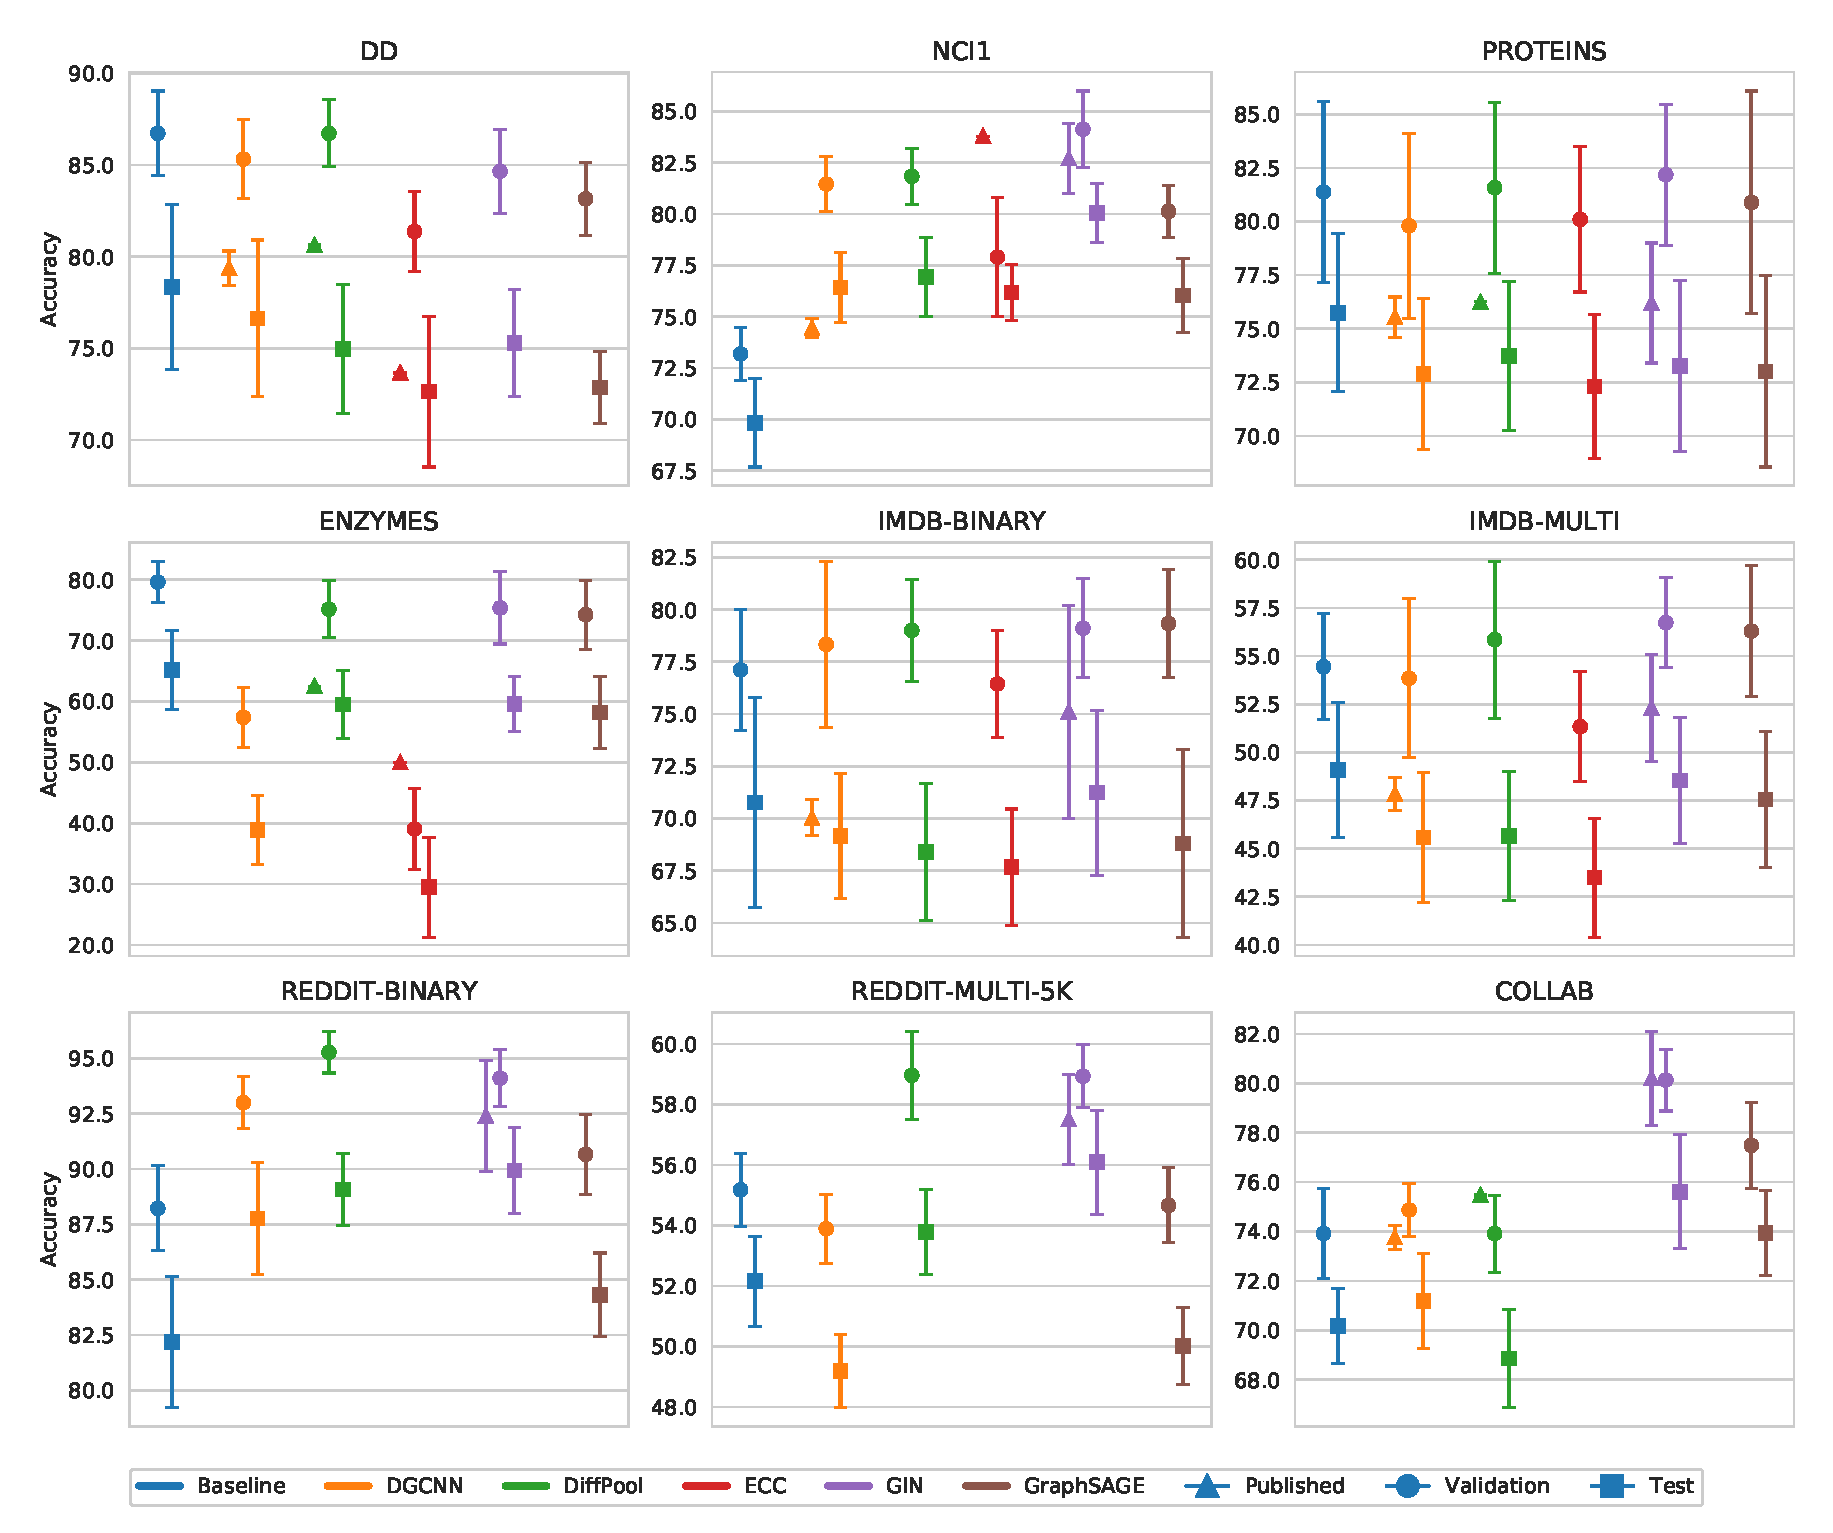
\includegraphics[width=\linewidth]{Figures/Chapter4/07-comparison-results.eps}
    \caption{Results.}
    \label{fig:comparison-plot}
\end{figure}
